% \section{Detached / Integrated AR library}
% \label{sect:input_handling}
When we started developing, none of us knew how Vuforia worked. Because of this
we had no specific plan for how we should handle the input. As we got into it,
we found that Vuforia gives us coordinates in space relative to the input
device / camera. From what we saw in the design document we wanted depth in the
games. We think this is logical since we try to combine the real 3D world with
our digital world presentation. Since we already got coordinates in space, we
thought that the input was convenient.

Nevertheless, the input did not fit our needs perfectly. In the "Total Sum"
game (\ref{game:total_sum}), we were building a tower to obtain the right
answer. I. e. "Combining Numbers" game (\ref{game:combining_numbers}) we were
putting cubes side by side in an horizontal fashion. We asked ourself how this
could be done when the camera could be all over the place.


\section{Different approaches}
One option could be to ask the player to have the camera only in one position
and then trust the user to obey our instructions. If trusting the user can be
avoided, we think we should. This relieves the user from potentially many
prerequisites. It also reduce the risk of complaint on the software when users
fail to follow the instructions and do not understand why the program doesn't
work as expected.

\paragraph{}

When we saw that the design document specified the creation of towers we came up with the idea to make use of the gyroscope that is found on many phones and tablets. The gyroscope allowed us to lock the input in to one or two axis for all the games. When the player was to build tower we could ignore horizontal connections and for all others we could ignore vertical connections. 

\paragraph{Frame-marker to cubes models}
Vuforia allows a small variety markers to give transforms(position, rotation and scale) to game-objects in unity. There is image-markers that can recognize an image even if it only sees a small part of the image. However the recommended max limit for image-markers was only five so at least for the cubes these were out of the question. There is also markers with shapes like cubes, cylinders, etc. but we had trouble getting these features to work, due to lack of documentation. And then there is the standard frame-marker which has to be completely visible to work but allows you to have up to 512 markers at once.\\
The standard way of using vuforia with unity is to set the gameObject to be a child of the marker in the game hierarchy. It will then be moved around, scale and rotate as the marker does and it will only be visible or active when the marker is recognized. This way does not allow the use more than one marker to find an object, markers cannot be children of each other. 

\begin{figure}[ht] 
        \capstart
        \centering  
        \includegraphics[width=\textwidth]{includes/simpleCubeMarkerModel.png}    
        \caption[Standard Cube-Marker model]{Simple visualization of the standard model.} 
        \label{fig:simple_cube_marker_model} 
\end{figure}

However you get very little control over it when you notice that the tracking is not quite as good as you want it to be. The cubes were jumpy, twitchy, disappear for a fraction of a frame and a few times even be consistently rotated more than 90 degrees off or remain on the screen long after the physical cube was taken away. The two last cases were quite rare and most of these could be blamed on the user not playing in optimal conditions or on the camera technology. But none the less it's a very volatile world to expose to algorithmic rules. We could not simply rely on the standard OnCollitionEnter, OnCollitionStay and  OnCollitionExit functions to handle the cubes connections. When a marker was lost, the virtual cube would disappear without calling OnCollitionExit(), leaving the program thinking the cubes were together when they may not have been. They were also so jumpy that they could make connections with cubes that weren't anywhere near them.\\
Our supervisor, Simon McCallum proposed the solution to separate the cubes and the markers to separate the volatile world from the game world. In the game world we could then freely manipulate it without changing the initial input. Also to make it easier to change the source of input so that we could quickly change the input to come from augmented reality glasses or from the web from someone else playing the game elsewhere instead of vuforia and the device camera.

\begin{figure}[ht] 
        \capstart
        \centering  
        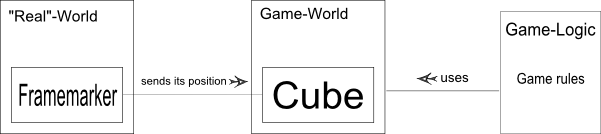
\includegraphics[width=\textwidth]{includes/complexCubeMarkerModel.png}    
        \caption[Separated Cube-Marker model]{Simple visualization of the separated model.} 
        \label{fig:complex_cube_marker_model} 
\end{figure}

In this model the markers would pass their transforms to the cubes as function parameters. The cubes would then use these to position them selfs in the game world. This model was not the one we went with but it had many options we had to consider:
\begin{itemize}
  \item We could use a different marker to show where the table is and use this to position and rotate the cubes. The cubes can not be lower than the table and they have to lay flat if they are on the table. Considering the instability of frame-markers (we couldn't just use one) and the difficulty of getting the markers recognized (we couldn't use many), frame-marker were pretty much out of the picture. We could use an image-target as a tablecloth. We tried to set up image-targets, but we couldn't get the targets recognized. It could have been a problem with the paper or size, scale, resolution of the image, lighting conditions, setup and so on, but we decided to drop this.
  \item We could have used more than one marker for each cube, put one on each side and average their transforms. This could have helped make the cubes just a little more visible and stable, but it would create a lot of complexity. Using several markers increases the chance of one of them, particularly the ones that are the least visible to mess up the cubes position even if it's not as much due to the averaging. The complexity would be a lot extra work for us to create handling for all those optional markers and for the devices that have to run the program. Since we were developing for tablets and cellphones we tried not to push the limits to much. It wouldn't help all that much since the cubes are massive objects, and really just need one clearly visible marker to be placed perfectly in the game world.
  \item We could handle the activation and deactivation of the cubes our selfs. This we did actually attempt to do. The result was a lot more stable, pretty and even colorful than the standard Vuforia- / Unityway, but much worse in relation to game-play. The cubes would freeze in place on the screen, for short periods of time making it hard to see what was going on behind them and generally just feel very unnatural to play with. We could have done the same as Vuforia to hide them when the markers aren't visible, but then there wouldn't really be a point in doing it and we didn't manage to make manual version as natural. 
  \item We could show transparent cubes where the markers were, manipulate the transforms and then place the cubes there with no transparency. But this would just be an excuse, a way to make up for the unnatural way of handling the input and it would probably just distract the player from the game it self.
\end{itemize}


\section{Solution}
In the end we decided to use the standard way, with a way to easier set different parents than the frame-markers and use filtering on the game-world state before testing for goal completion, rather than modifying the cubes positions before displaying them to the user. We found this gave the cubes fairly natural and more relate-able and forgivable behavior and to be better for playing the game as players. This way shows the player the instable recognition of the markers, allowing him to adapt to it while keeping the world state that is being tested with the game rules to be a little more stable than it seems. Not by using individual manipulation, but by universal filtering to make the state stable.